\section{Case Studies}
\label{surface_reconstruction_section_case_studies}

The surface reconstruction problem being inherently ill-posed, the proposed algorithm does not pretend to reconstruct all kinds of surfaces with arbitrary sampling conditions. This section provides the user with some hints about the ideal sampling and contouring conditions, and depicts some failure cases when these conditions are not matched.

\subsection{Ideal Conditions}

The user must keep in mind that the poisson surface reconstruction algorithm comprises two phases (computing the implicit function from the input point set and contouring an iso-surface of this function). Both require some care in terms of sampling conditions and parameter tuning.

\subsubsection{Point Set}

Ideally the current implementation of the Poisson surface reconstruction method expects a dense 3D oriented point set (typically matching the epsilon-sampling condition~\cite{cgal:bo-pgsms-05}) and sampled over a closed, smooth surface. Oriented herein means that all 3D points must come with consistently oriented normals to the inferred surface. Figures \ref{Surface_reconstruction_points_3-fig-bimba} and \ref{Surface_reconstruction_points_3-fig-eros} illustrate cases where these ideal conditions are met.

% Insert image bimba.png/.eps
\begin{center}
    \label{Surface_reconstruction_points_3-fig-bimba}
    \begin{ccTexOnly}
  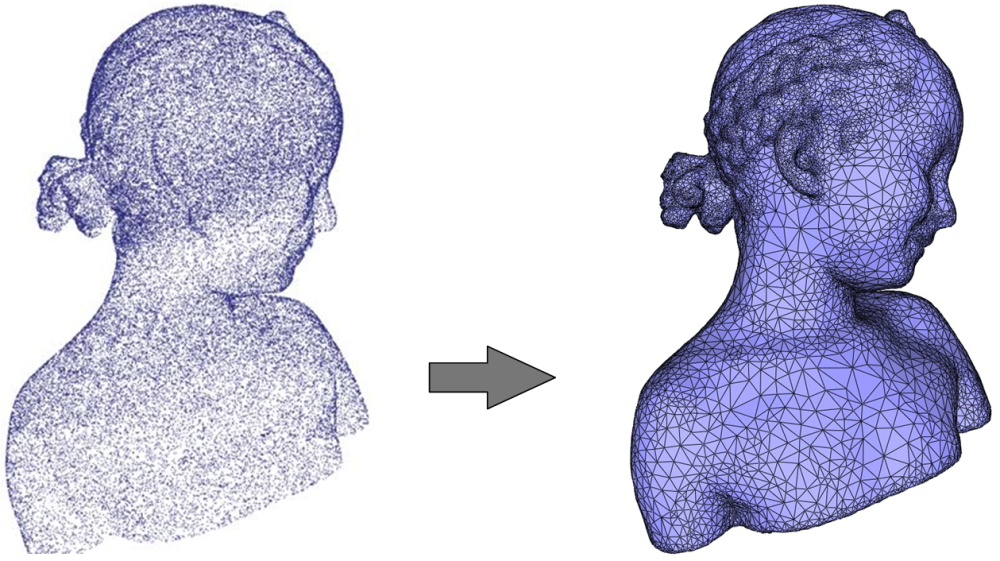
\includegraphics[width=1.0\textwidth]{Surface_reconstruction_points_3/bimba}
    \end{ccTexOnly}
    \begin{ccHtmlOnly}
        <img width="80%" border=0 src="./bimba.png"><P>
    \end{ccHtmlOnly}
    \begin{figure}[h]
        \caption{Poisson reconstruction.
                 Left: 120K points sampled on a statue (Minolta laser scanner).
                 Right: reconstructed surface mesh.}
    \end{figure}
\end{center}

% Insert image eros.png/.eps
\begin{center}
    \label{Surface_reconstruction_points_3-fig-eros}
    \begin{ccTexOnly}
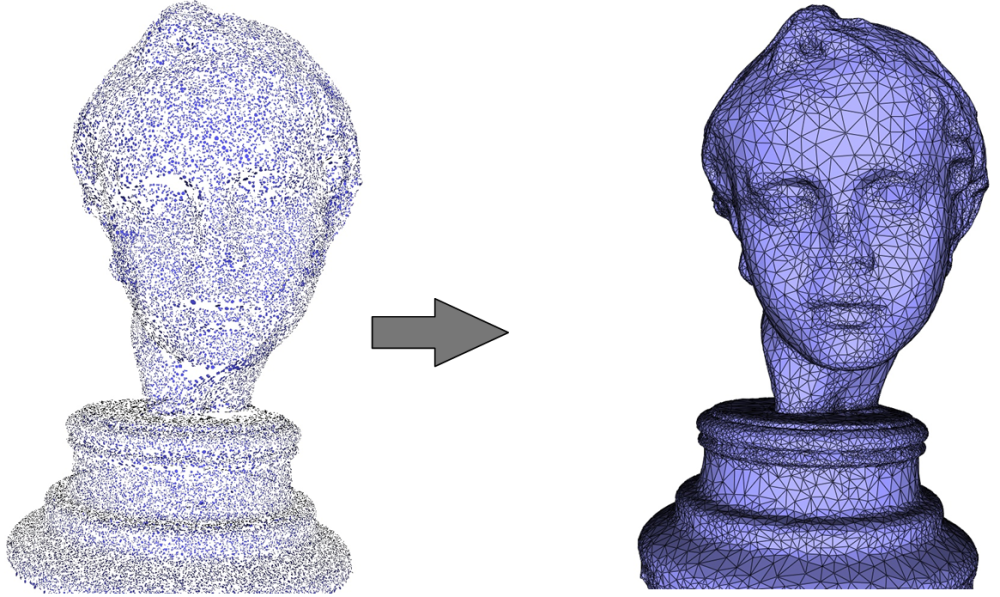
\includegraphics[width=1.0\textwidth]{Surface_reconstruction_points_3/eros}
    \end{ccTexOnly}
    \begin{ccHtmlOnly}
        <img width="80%" border=0 src="./eros.png"><P>
    \end{ccHtmlOnly}
    \begin{figure}[h]
        \caption{Left: 120K points sampled on a statue (Minolta laser scanner).
                 Right: reconstructed surface mesh.}
    \end{figure}
\end{center}

The algorithm is fairly robust to anisotropic sampling and to noise. It is also robust to missing data through filling the corresponding holes as the algorithm is designed to reconstruct the indicator function of an inferred solid (see Figure~\ref{Surface_reconstruction_points_3-fig-holes_good}).

% Insert image holes_good.png/.eps
\begin{center}
    \label{Surface_reconstruction_points_3-fig-holes_good}
    \begin{ccTexOnly}
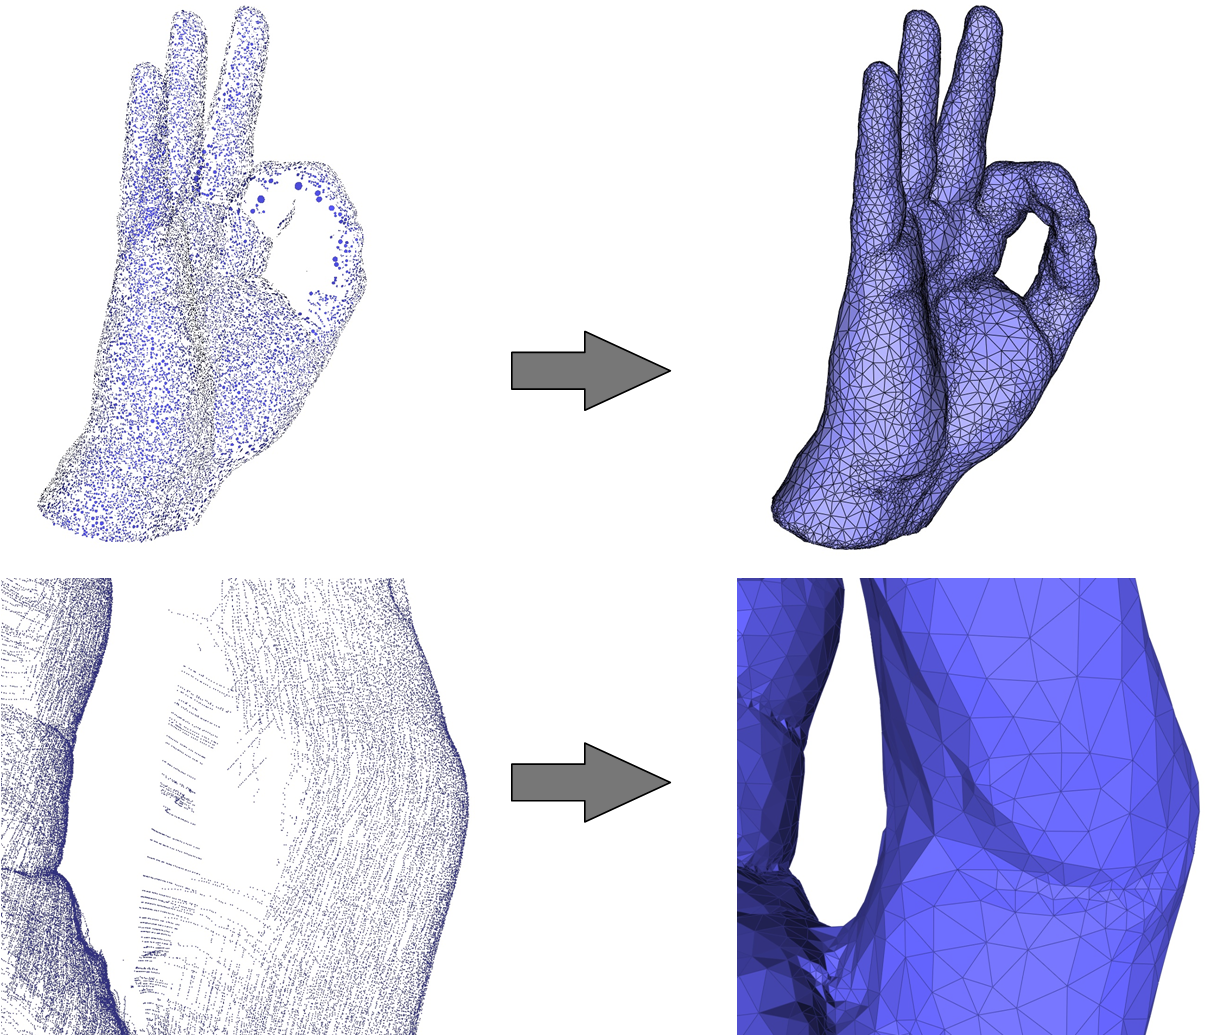
\includegraphics[width=1.0\textwidth]{Surface_reconstruction_points_3/holes_good}
    \end{ccTexOnly}
    \begin{ccHtmlOnly}
        <img width="80%" border=0 src="./holes_good.png"><P>
    \end{ccHtmlOnly}
    \begin{figure}[h]
        \caption{Top left: 65K points sampled on a hand (Kreon laser scanner).
                 Bottom left: the point set is highly anisotropic due
                 to the scanning technology.
                 Right: reconstructed surface mesh and closeup.
                 The holes are properly closed.}
    \end{figure}
\end{center}

The algorithm is in general not robust to outliers, although a few outliers do not always create a failure, see Figure~\ref{Surface_reconstruction_points_3-fig-outliers}.

% Insert image outliers.png/.eps
\begin{center}
    \label{Surface_reconstruction_points_3-fig-outliers}
    \begin{ccTexOnly}
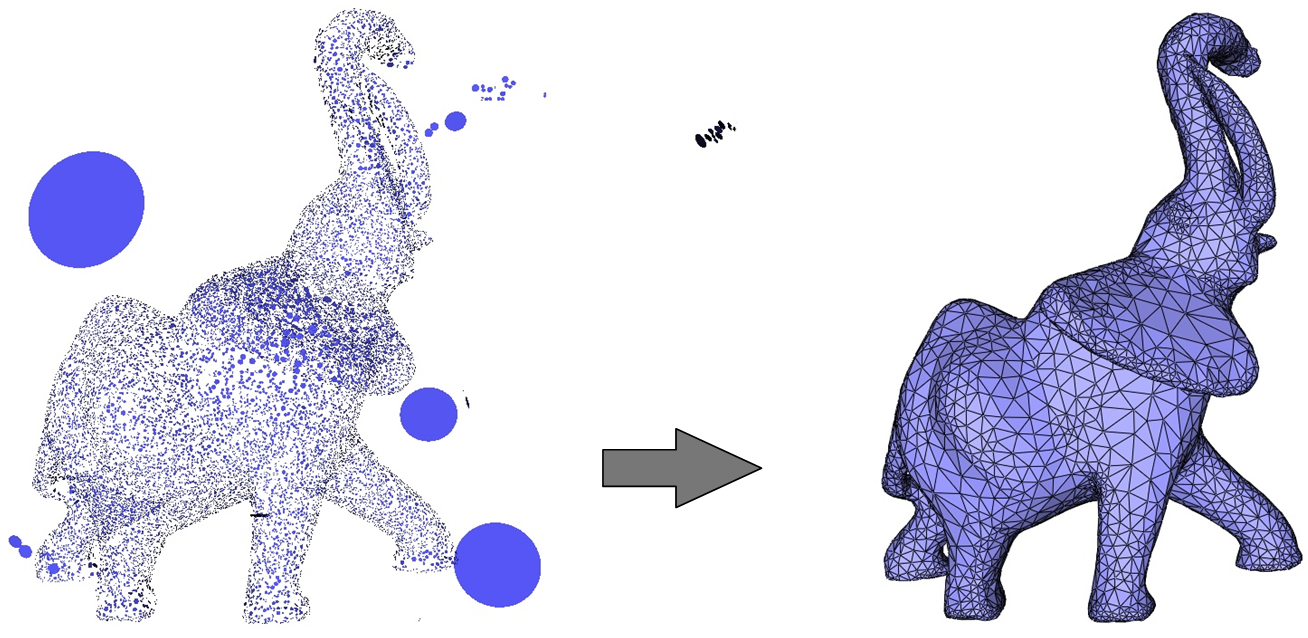
\includegraphics[width=1.0\textwidth]{Surface_reconstruction_points_3/outliers}    \end{ccTexOnly}
    \begin{ccHtmlOnly}
        <img width="80%" border=0 src="./outliers.png"><P>
    \end{ccHtmlOnly}
    \begin{figure}[h]
        \caption{Left: 70K points sampled on an elephant with few
                 outliers emphasized with circles.
                 % careful: show circles not disks
                 Right: reconstructed surface mesh.}
    \end{figure}
\end{center}


The algorithm works well even when the inferred surface is composed of several connected components, provided that both all normals are properly estimated and oriented (the current CGAL normal orienter algorithm may fail in some cases, see \ccc{CGAL::mst_orient_normals()}), and that the final contouring algorithm is properly seeded for each component. When the inferred surface is composed of several nested connected components care should be taken to orient the normals of each component in alternation (inward/outward) so that the final contouring stage picks a proper contouring value. 
    

\subsubsection{Contouring Parameters}

Our implementation of the Poisson surface reconstruction algorithm computes an implicit function represented as a piecewise linear function over the tetrahedra of a 3D Delaunay triangulation constructed from the input points then refined through Delaunay refinement. For this reason any iso-surface is also piecewise linear and hence may contain sharp creases. As the contouring algorithm \ccc{CGAL::make_surface_mesh()} expects a smooth implicit function these sharp creases may create spurious clusters of vertices in the final reconstructed surface mesh when setting a small mesh sizing or surface approximation error parameter (see Figure~\ref{Surface_reconstruction_points_3-fig-contouring_bad}). One way to avoid these spurious clusters consists of adjusting the mesh sizing and surface approximation parameters large enough compared to the average sampling density (obtained through \ccc{CGAL::compute_average_spacing()}) so that the contouring algorithm ``perceives'' a smooth iso-surface. We recommend to use the following contouring parameters:
\begin{itemize}
\item Max triangle radius: at least 100 times the average spacing.
\item Approximation distance: at least 0.25 times the average spacing.
\end{itemize}

% PA: we are missing the number of input points here.
% Insert image contouring_bad.png/.eps
\begin{center}
    \label{Surface_reconstruction_points_3-fig-contouring_bad}
    \begin{ccTexOnly}
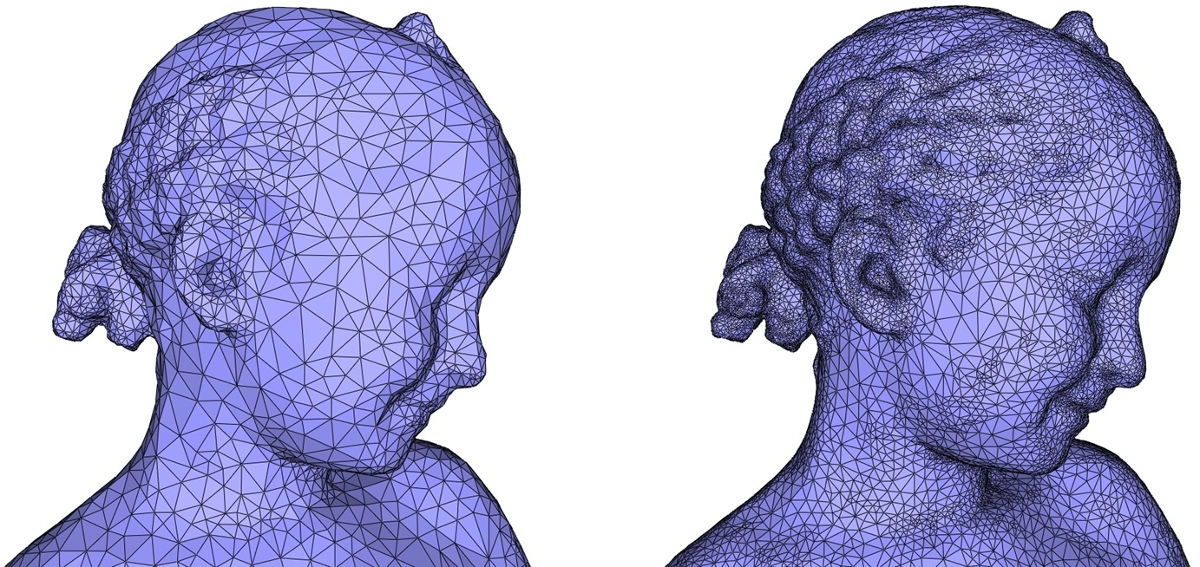
\includegraphics[width=1.0\textwidth]{Surface_reconstruction_points_3/contouring_bad}
    \end{ccTexOnly}
    \begin{ccHtmlOnly}
        <img width="80%" border=0 src="./contouring_bad.png"><P>
    \end{ccHtmlOnly}
    \begin{figure}[h]
        \caption{Left: surface reconstructed with approximation distance = 0.25 * average spacing.
                 Right: surface reconstructed with approximation distance = 0.15 * average spacing. Notice the spurious cluster on the chick.}
    \end{figure}
\end{center}


\subsection{Degraded Conditions}

\subsubsection{Holes}

By construction, this method contours the zero level set of an implicit function and reconstructs a closed mesh.\\
For small holes, this is probably what you expect. \\
In case of large holes that you do not want to close or that you want to close with a plane, you will need a postprocessing stage.

% Insert image holes_bad.png/.eps
\begin{center}
    \label{Surface_reconstruction_points_3-fig-holes_bad}
    % Image
    \begin{ccTexOnly}
      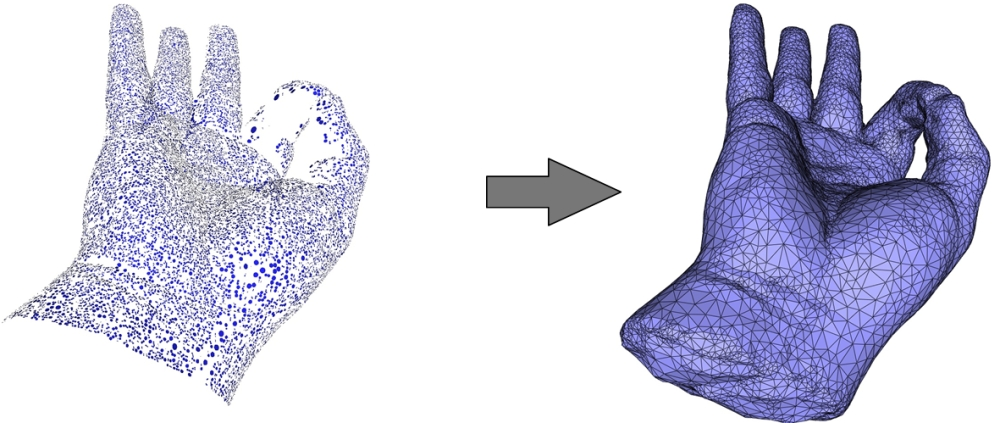
\includegraphics[width=0.5\textwidth]{Surface_reconstruction_points_3/holes_bad} % omit .eps suffix
    \end{ccTexOnly}
    \begin{ccHtmlOnly}
        <img width="50%" border=0 src="./holes_bad.png"><P>
    \end{ccHtmlOnly}
    % Title
    \begin{figure}[h]
        \caption{Left: 65K points sampled on hand with no data captured at the wrist base.
                 Right: reconstructed surface mesh. Notice that surface is properly closed on the fingers
                 but also closed at the wrist in a non-natural way.}
    \end{figure}
\end{center}


\subsubsection{Noise}

Poisson reconstruction method supports noise if the approximation distance requested at the contouring stage is large w.r.t. the noise.\\
If you wish to use a small approximation distance, you may remove noise as a preprocessing step using \ccc{CGAL::jet_smooth_point_set()}.

% Insert image noise.png/.eps
\begin{center}
    \label{Surface_reconstruction_points_3-fig-noise}
    % Image
    \begin{ccTexOnly}
      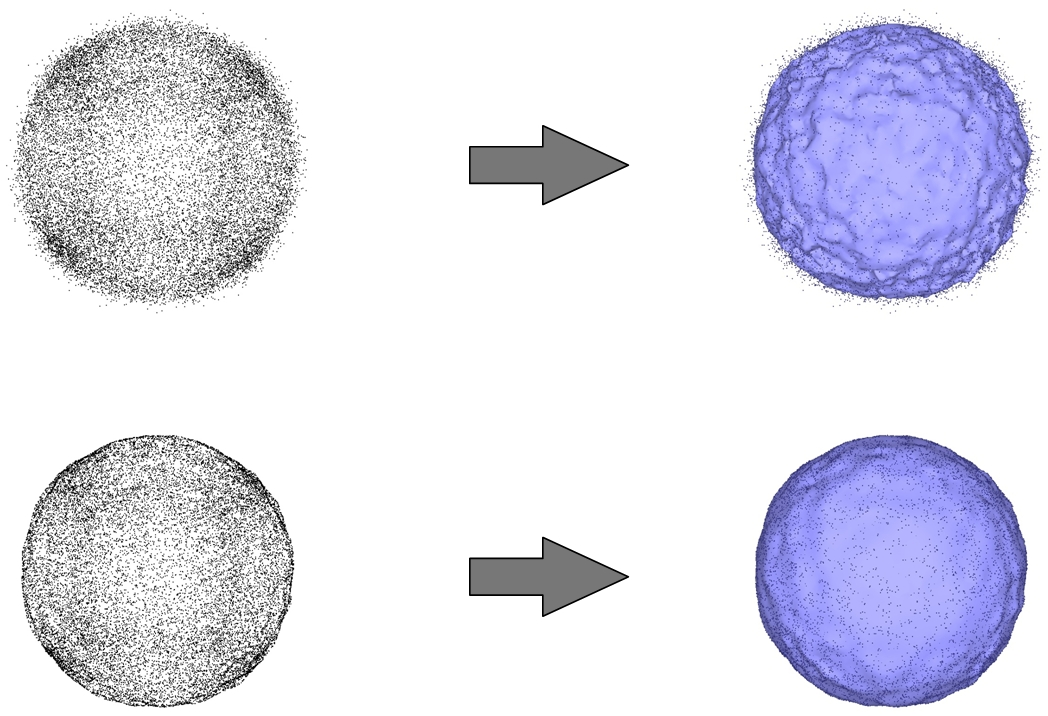
\includegraphics[width=0.5\textwidth]{Surface_reconstruction_points_3/noise} % omit .eps suffix
    \end{ccTexOnly}
    \begin{ccHtmlOnly}
        <img width="50%" border=0 src="./noise.png"><P>
    \end{ccHtmlOnly}
    % Title
    \begin{figure}[h]
        \caption{Top-left: points sampled on sphere with a lot of noise.
                 Top-right: reconstructed surface mesh. Notice the bumps.
                 Bottom-left: smoothed point set.
                 Bottom-right: reconstructed surface mesh.}
    \end{figure}
\end{center}


\subsubsection{Outliers}

Poisson reconstruction method supports a small amount of outliers (see elephant example above).\\
Large clusters of outliers should be removed as a preprocessing step using \ccc{CGAL::remove_outliers()}.


\subsubsection{Sampling}

Poisson surface reconstruction method expects a dense point set, respecting the epsilon-sampling condition:
the input points spacing must be 10 times smaller than the local feature size. When this condition is not respected, the reconstruction may miss thin undersampled regions.

% Insert image sampling.png/.eps
\begin{center}
    \label{Surface_reconstruction_points_3-fig-sampling}
    % Image
    \begin{ccTexOnly}
      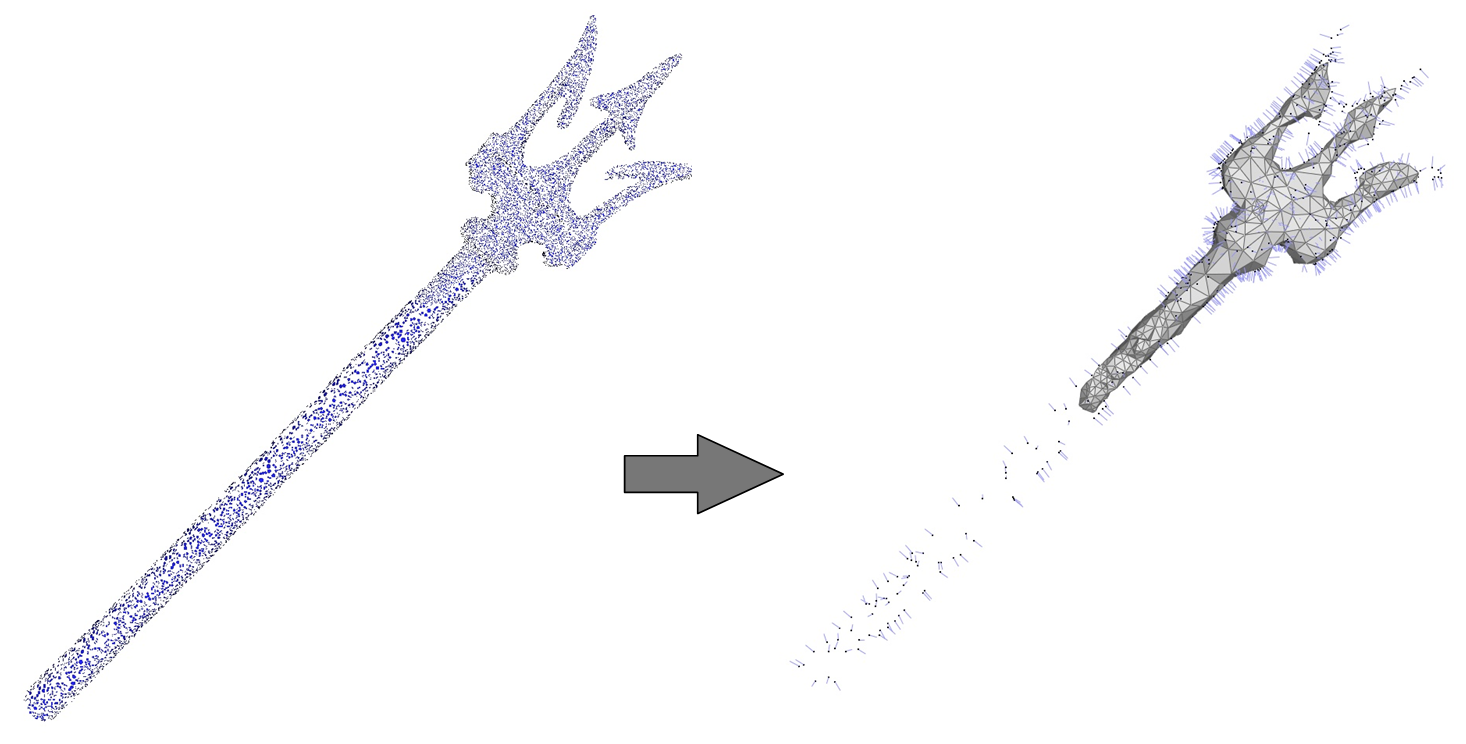
\includegraphics[width=0.5\textwidth]{Surface_reconstruction_points_3/sampling} % omit .eps suffix
    \end{ccTexOnly}
    \begin{ccHtmlOnly}
        <img width="50%" border=0 src="./sampling.png"><P>
    \end{ccHtmlOnly}
    % Title
    \begin{figure}[h]
        \caption{Left: 50K points sampled on a Neptune trident.
                 Right: point set simplified to 1K and then reconstructed
                 (input points are drawn with normals to show the missed region).}
    \end{figure}
\end{center}


\subsubsection{Normals}

As Poisson surface reconstruction solves a global linear system in the least square sense, it supports isolated flipped normals.
On the other hand, a cluster of wrong normals will lead to an incorrect implicit function.

% Insert image flipped_normals.png/.eps
\begin{center}
    \label{Surface_reconstruction_points_3-fig-flipped_normals}
    % Image
    \begin{ccTexOnly}
      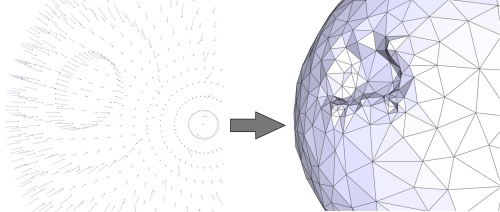
\includegraphics[width=0.5\textwidth]{Surface_reconstruction_points_3/flipped_normals} % omit .eps suffix
    \end{ccTexOnly}
    \begin{ccHtmlOnly}
        <img width="50%" border=0 src="./flipped_normals.png"><P>
    \end{ccHtmlOnly}
    % Title
    \begin{figure}[h]
        \caption{Left: points sampled on a sphere with a cluster of flipped normals.
                 Right: reconstructed surface mesh. Notice the bump in the surface.}
    \end{figure}
\end{center}


\subsubsection{Sharp Features}

Poisson surface reconstruction does not support sharp features.

% Insert image sharp_features.png/.eps
\begin{center}
    \label{Surface_reconstruction_points_3-fig-sharp_features}
    % Image
    \begin{ccTexOnly}
      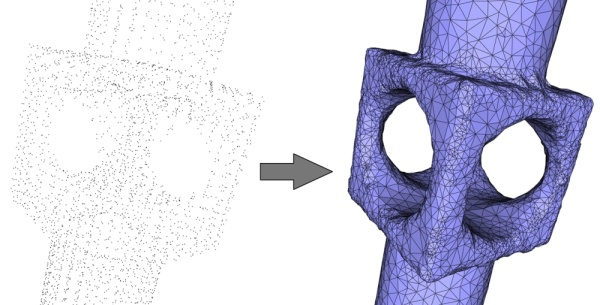
\includegraphics[width=0.5\textwidth]{Surface_reconstruction_points_3/sharp_features} % omit .eps suffix
    \end{ccTexOnly}
    \begin{ccHtmlOnly}
        <img width="50%" border=0 src="./sharp_features.png"><P>
    \end{ccHtmlOnly}
    % Title
    \begin{figure}[h]
        \caption{Left: 5K points sampled on a mechanical piece.
                 Right: reconstructed surface mesh. Notice that sharp edges are smoothed.}
    \end{figure}
\end{center}


\subsubsection{Several Connected Components}

This package does not support point sets with several clusters of points. The main limitation is that \ccc{CGAL::mst_orient_normals()} cannot orient coherently the normals of several clusters of points. The contouring phase (i.e. the call to \ccc{make_surface_mesh()}) also requires a different initialization to handle several connected components.

